\chapter{Desarrollo iterativo}
\label{chap:desarrollo-iterativo}

\section{Sprint 1: cimientos y esqueleto autenticado}

El incremento comenzó con una solución .NET y dos proyectos independientes, más una SPA TypeScript. En backend se implementaron la entidad de usuario, su configuración EF Core y la migración \texttt{InitialCreate}; el servicio de autenticación; los controladores de salud y sesión; JWT, CORS, correlación y tratamiento uniforme de excepciones.

En frontend se construyeron el cliente HTTP, un contexto de sesión persistente, la pantalla de login, el componente de error, la ruta protegida y un layout adaptable. Un administrador ve la futura entrada de usuarios, mientras que un operador recibe solo la navegación común. El resultado atraviesa navegador, proxy, API y PostgreSQL: constituye un \gls{walking-skeleton} real.

Docker Compose orquesta base de datos, API y web; la API aplica migraciones al arrancar. GitHub Actions compila y prueba ambas aplicaciones y ejecuta la migración contra PostgreSQL. Esta infraestructura se mantendrá en todos los incrementos siguientes.

\begin{figure}[htbp]
\centering
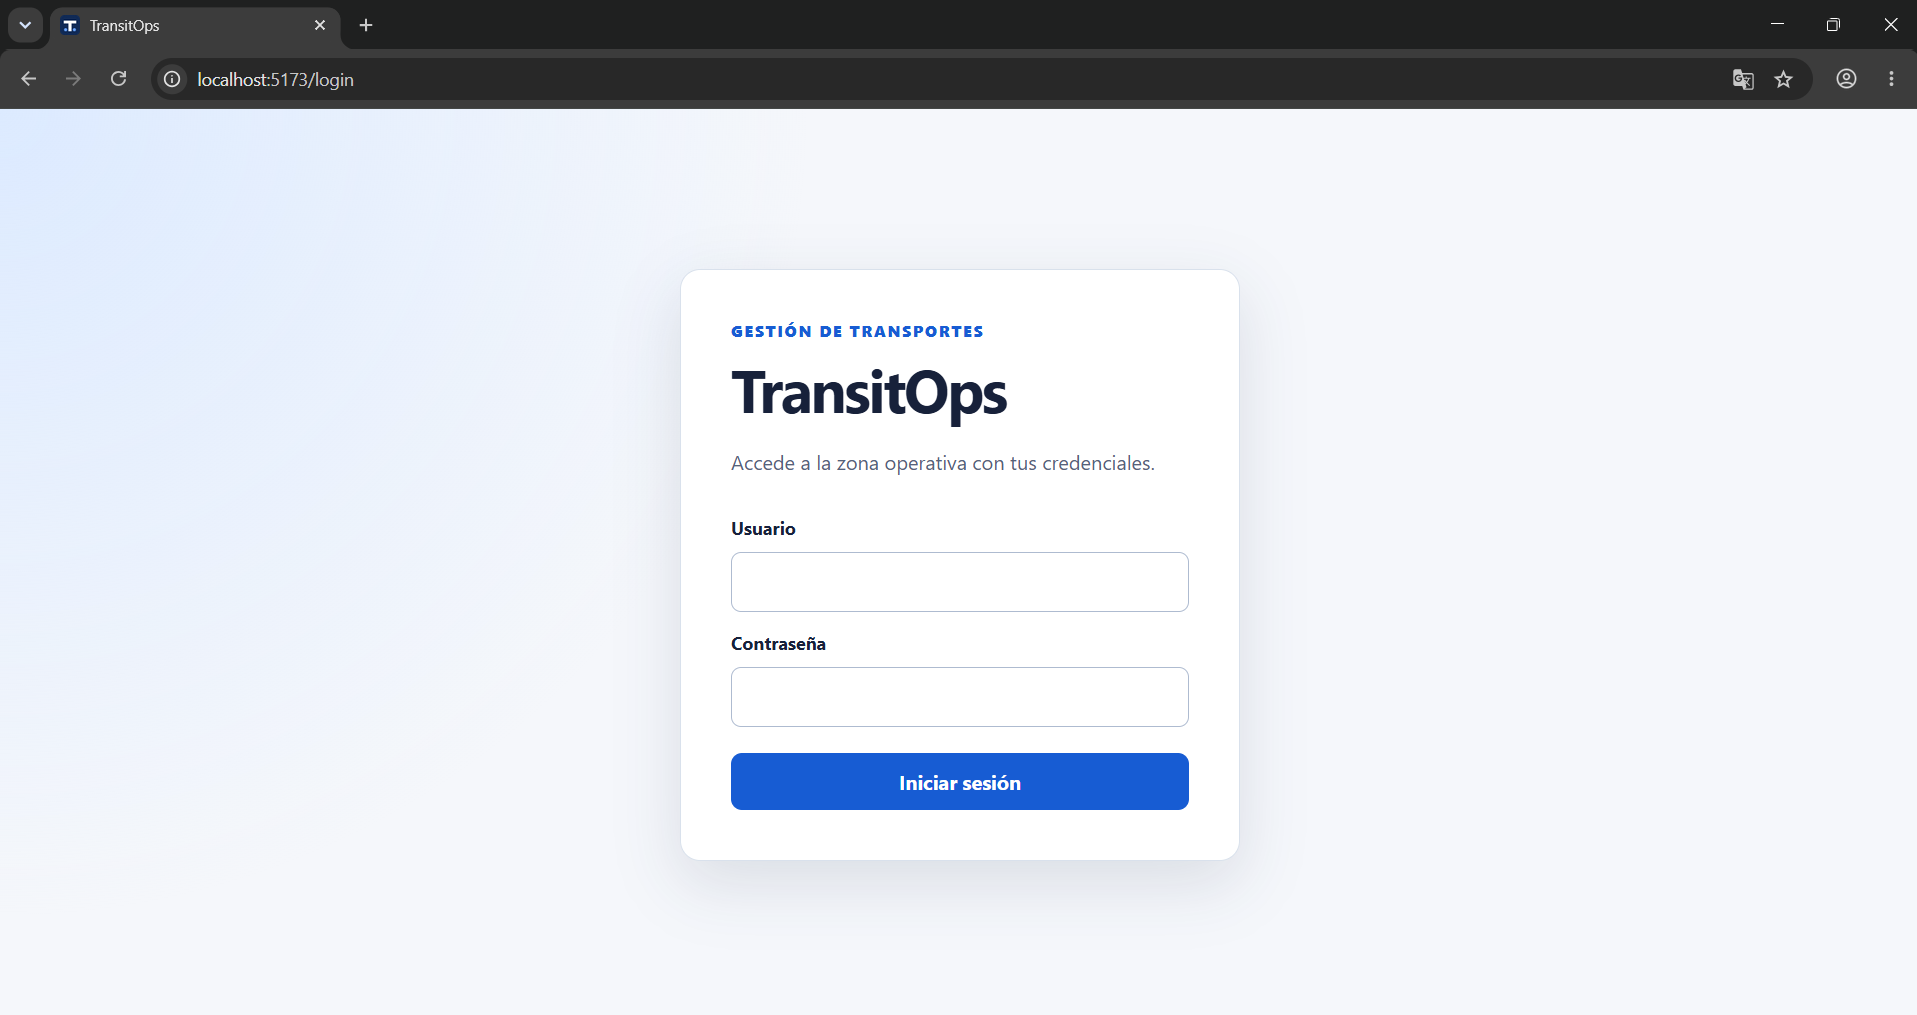
\includegraphics[width=0.8\textwidth]{imaxes/login-docker-compose}
\caption{Pantalla de login servida por el stack de Docker Compose}
\label{fig:login-compose}
\end{figure}

\section{Sprint 2: catálogos operativos}

El segundo incremento incorporó vehículos, conductores y clientes como tres rebanadas coherentes. Cada catálogo dispone de listado, detalle, alta, edición y baja lógica tanto en la API como en la SPA. Los identificadores de negocio de vehículos y conductores se normalizan y son únicos entre registros activos, de modo que una baja conserva el historial y permite reutilizar el identificador.

La migración \texttt{AddCatalogTables} llevó el diseño a PostgreSQL sin alterar la autenticación existente. Los formularios reutilizan el contrato común de validación y muestran los conflictos junto al flujo que los origina. El cierre dejó 29 pruebas backend y 7 frontend correctas y verificó el flujo real a través de Nginx, API y PostgreSQL.

\section{Sprint 3: envíos y visibilidad operativa}

El tercer incremento añadió el agregado \texttt{Shipment}. Cada envío tiene una referencia única global, origen, destino y recogida prevista obligatorios; puede asociar cliente, entrega prevista, carga estimada y notas. Nace siempre planificado y no admite borrado: el ciclo de estados se abordará en el incremento siguiente. Las claves foráneas restrictivas preservan los vínculos históricos con los catálogos.

La API normaliza referencias y fechas antes de persistir o filtrar. Los instantes se almacenan como UTC en \texttt{timestamp with time zone}; las entradas sin zona se interpretan según el contrato como UTC y las que incluyen desplazamiento conservan el instante. La regla que impide una entrega anterior a la recogida se comprueba en el contrato HTTP, el servicio y la base de datos.

La SPA ofrece alta, edición, detalle y una tabla paginada. Los filtros de estado, rango de recogida, vehículo y conductor viven en la URL. El formulario convierte de forma explícita entre \texttt{datetime-local} y UTC, muestra los errores por campo y conserva la asociación visible al editar un envío cuyo cliente ya fue dado de baja.

La automatización del cierre alcanzó 45 pruebas backend y 13 frontend, con compilaciones de producción y análisis estático correctos.

\begin{figure}[htbp]
\centering
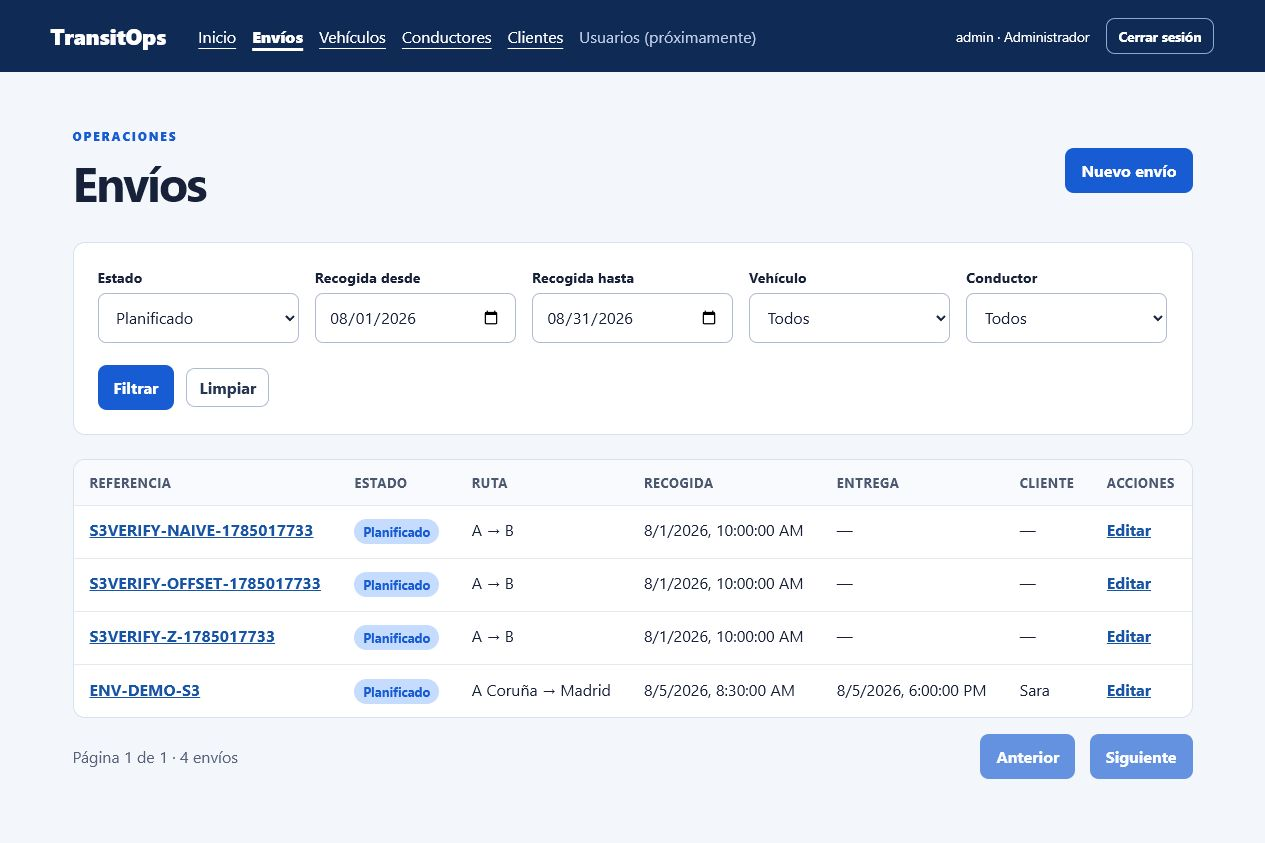
\includegraphics[width=\textwidth]{imaxes/envios-filtrados-sprint3}
\caption{Listado de envíos con filtros de estado y fecha persistidos en la URL}
\label{fig:envios-filtrados-s3}
\end{figure}

\begin{figure}[htbp]
\centering
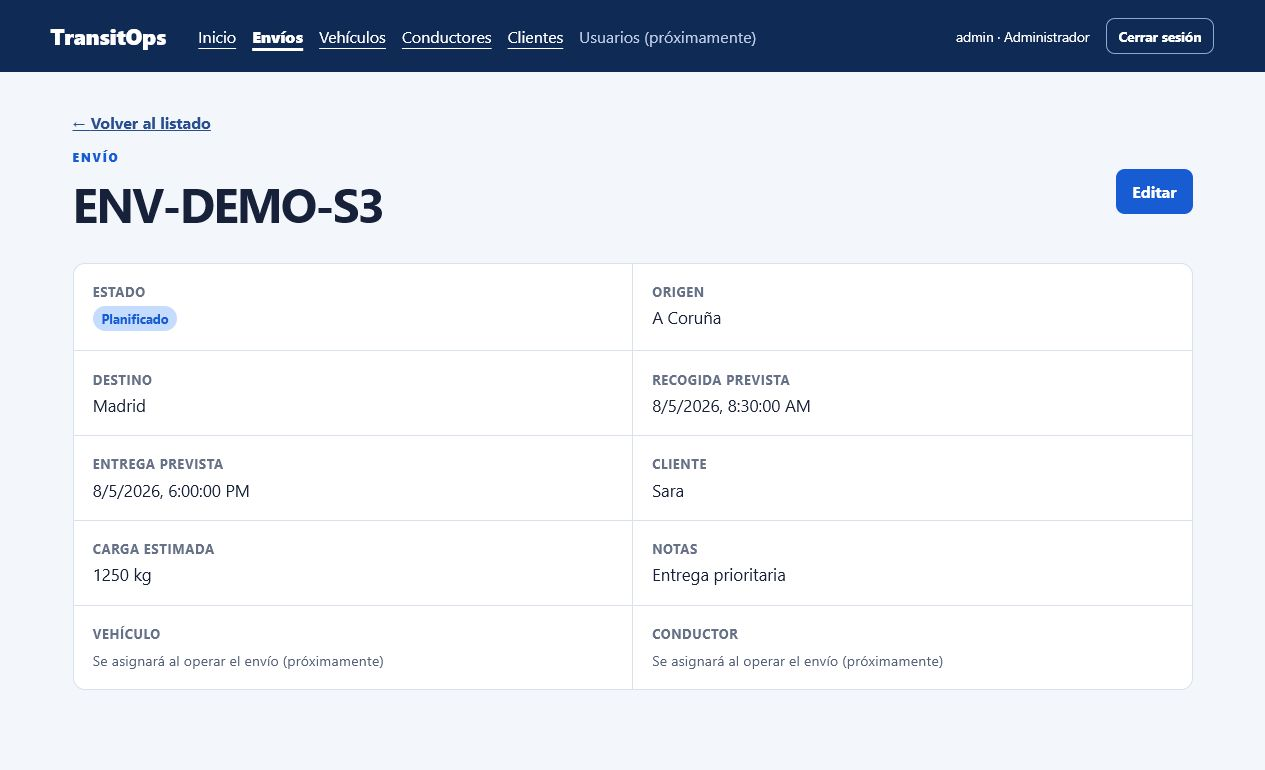
\includegraphics[width=\textwidth]{imaxes/envio-detalle-sprint3}
\caption{Detalle de un envío planificado con cliente y carga estimada}
\label{fig:envio-detalle-s3}
\end{figure}

\clearpage
\section{Sprint 4: asignación y ciclo de vida}

El cuarto incremento convirtió el detalle del envío en la pantalla de operación. La asignación trata vehículo y conductor como una unidad y solo se modifica mientras el envío está planificado. El servicio rechaza recursos inexistentes o dados de baja y consulta el resto de envíos planificados o en curso para impedir una doble reserva. La consulta excluye el propio envío, por lo que es posible cambiar únicamente el conductor sin provocar un falso conflicto con el vehículo que ya tenía asignado.

La capacidad insuficiente sigue una semántica distinta a la de los errores: la asignación se persiste y la respuesta incorpora un aviso transitorio. La SPA lo muestra en ámbar, separado del componente rojo de error. No se persiste una bandera derivada que podría quedar obsoleta al editar la carga o el vehículo.

La máquina de estados adopta una política cerrada: solo se permiten las cuatro transiciones dibujadas en la Figura~\ref{fig:maquina-estados-s4}. Entrar en curso requiere los dos recursos y sella la recogida real en UTC; entregar sella la entrega real. Entregado y cancelado son terminales, y ninguna operación devuelve el envío a planificado.

La migración \texttt{AddShipmentOperation} añadió las dos fechas reales y una restricción de coherencia. La API expone acciones explícitas para asignar, retirar la asignación y cambiar el estado; el CRUD general no puede alterar estos campos. En la interfaz, los botones se derivan del estado actual, las acciones irreversibles piden confirmación y un estado final muestra de forma explícita que ya no admite cambios.

\begin{figure}[htbp]
\centering
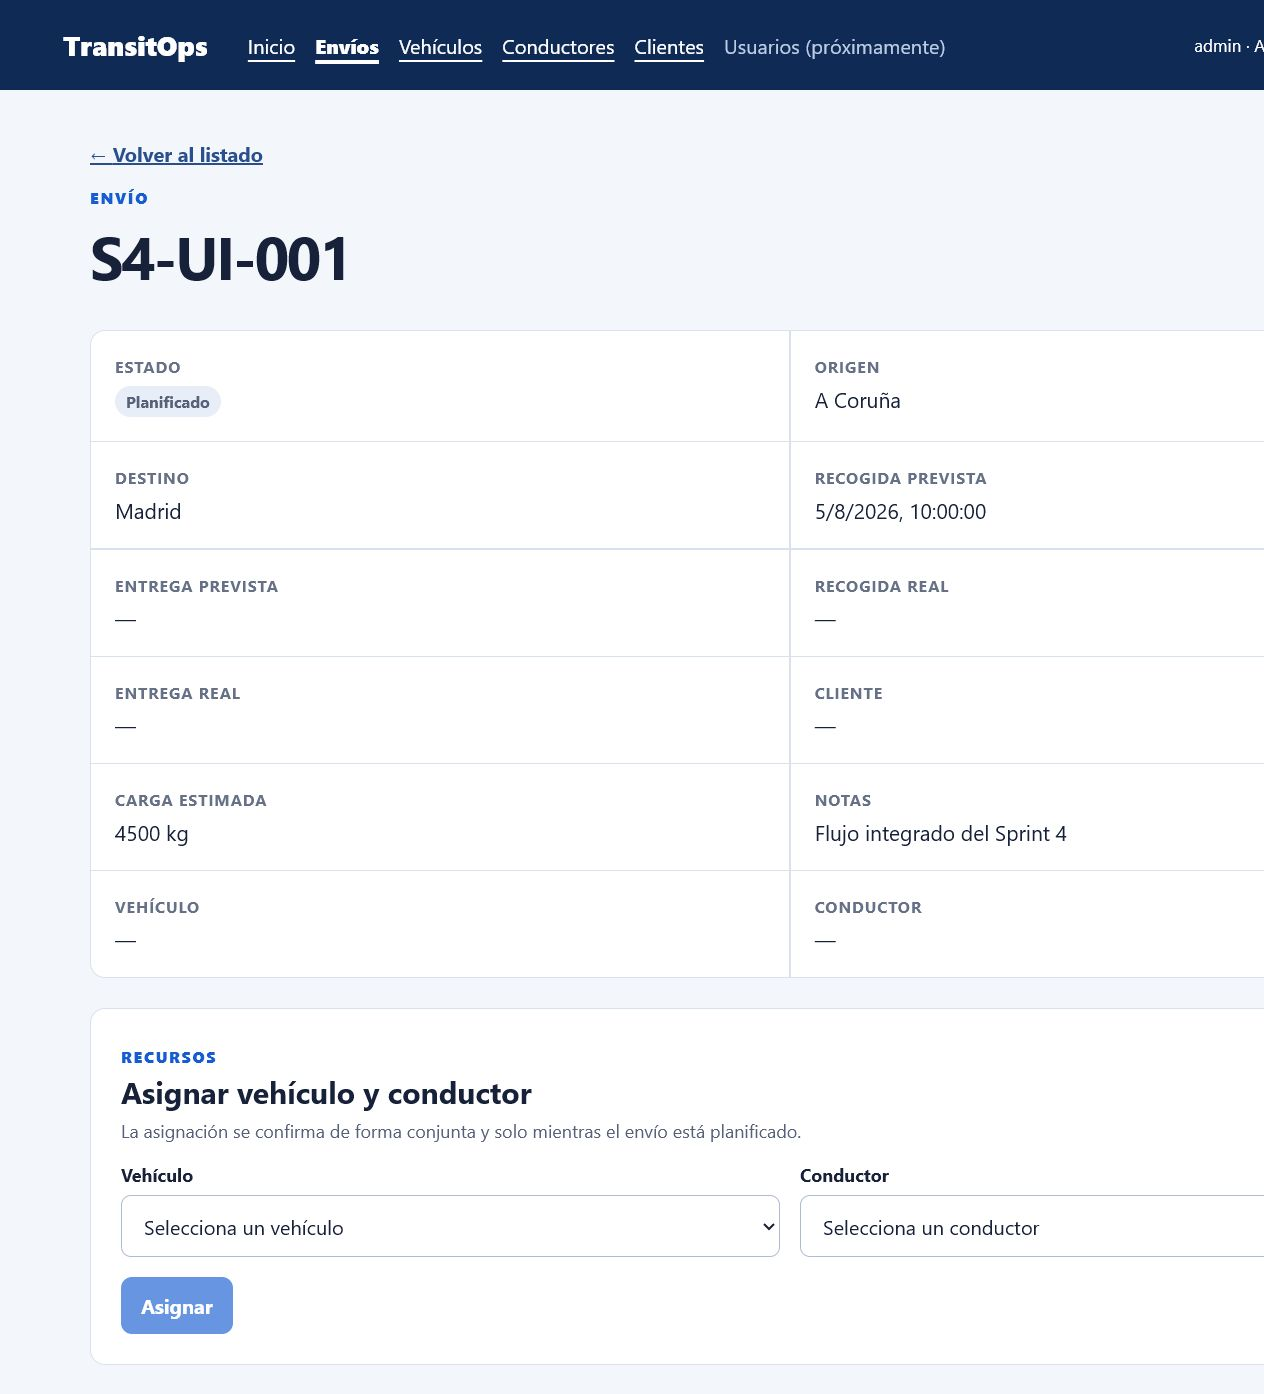
\includegraphics[width=0.72\textwidth]{imaxes/envio-planificado-sprint4}
\caption{Panel conjunto de asignación en un envío planificado}
\label{fig:asignacion-s4}
\end{figure}

\begin{figure}[htbp]
\centering
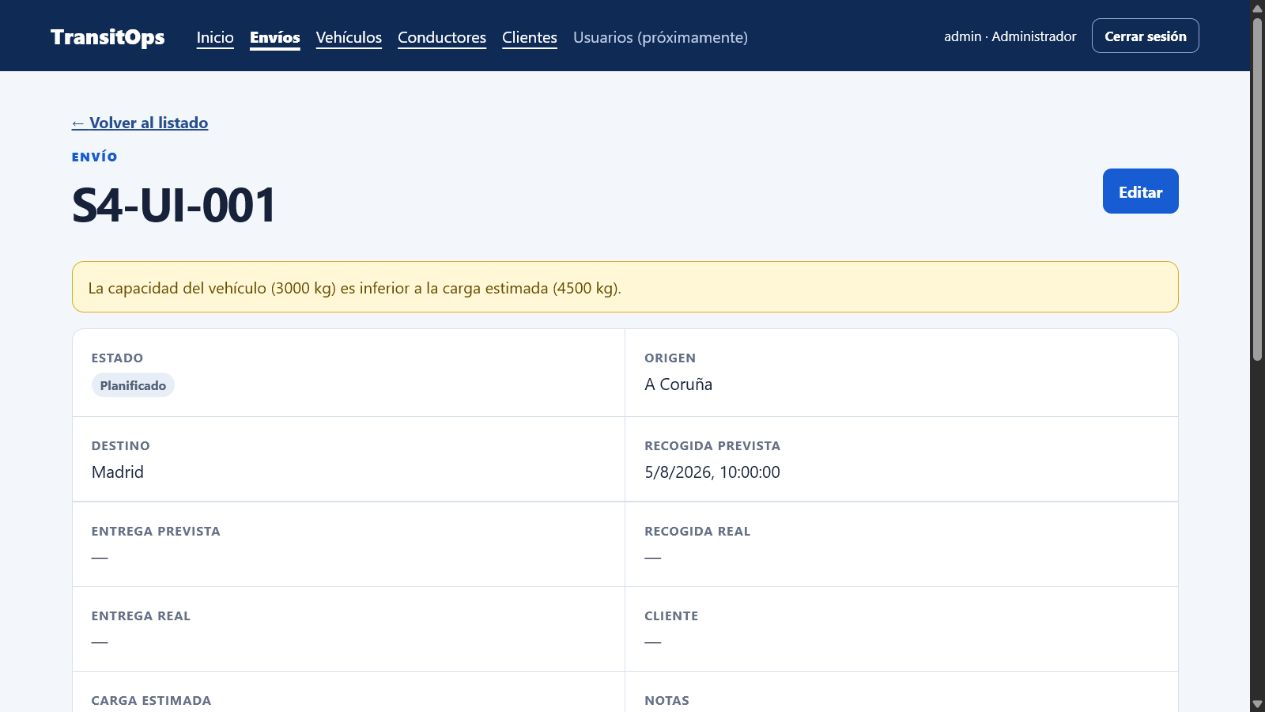
\includegraphics[width=\textwidth]{imaxes/aviso-capacidad-sprint4}
\caption{Asignación guardada con aviso no bloqueante de capacidad}
\label{fig:capacidad-s4}
\end{figure}

\begin{figure}[htbp]
\centering
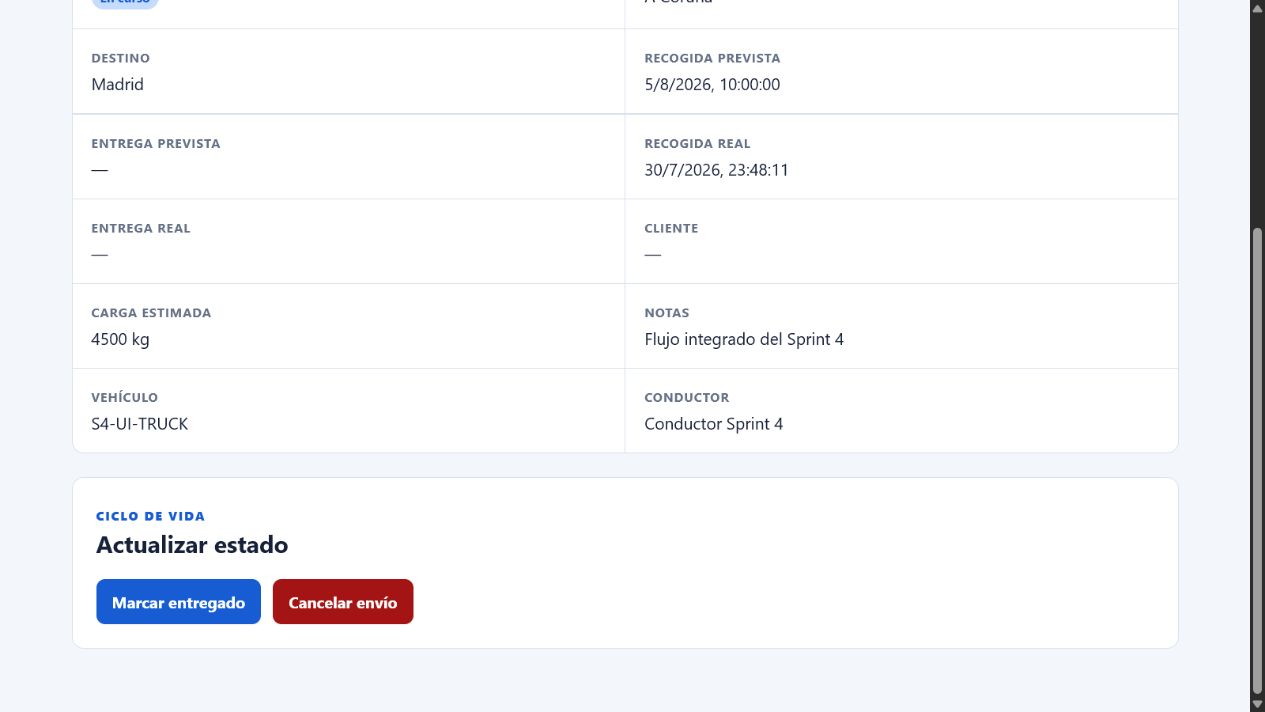
\includegraphics[width=\textwidth]{imaxes/envio-en-curso-sprint4}
\caption{Envío en curso con recogida real y acciones válidas}
\label{fig:en-curso-s4}
\end{figure}

\begin{figure}[htbp]
\centering
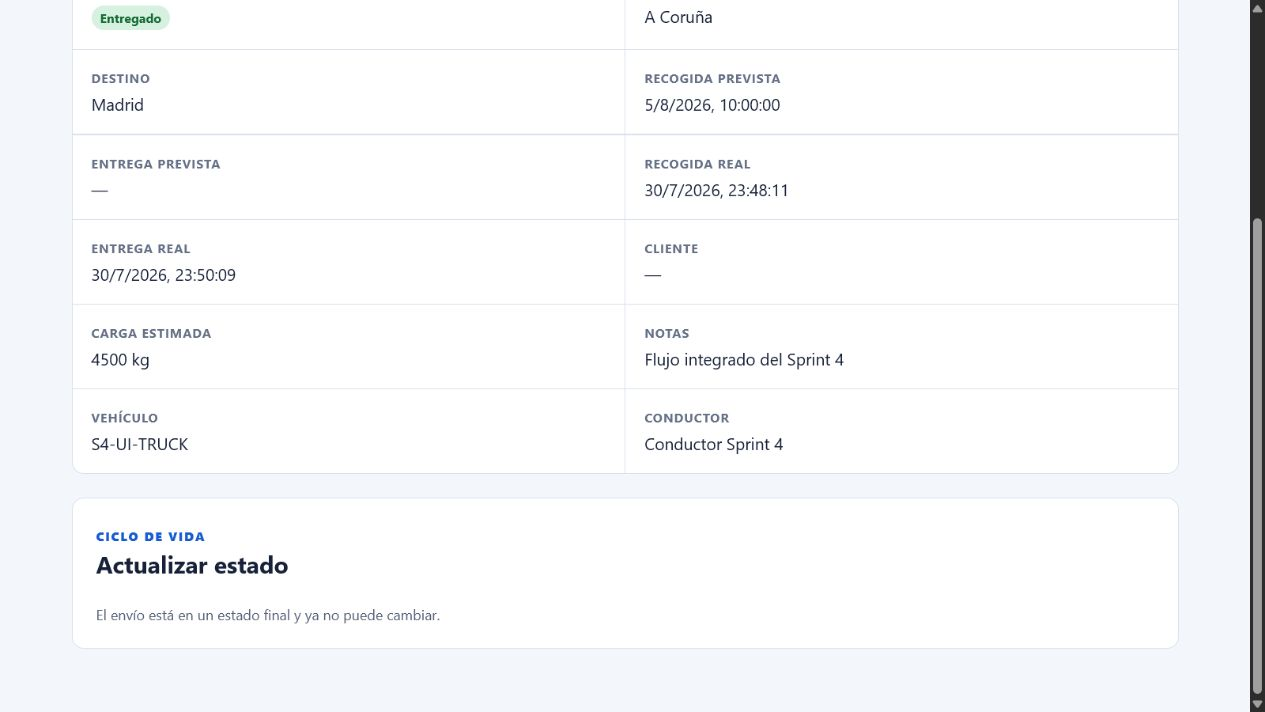
\includegraphics[width=\textwidth]{imaxes/envio-entregado-sprint4}
\caption{Envío entregado, con fechas reales y sin acciones de transición}
\label{fig:entregado-s4}
\end{figure}

\clearpage
\section{Sprint 5: trazabilidad de eventos}

El quinto incremento completó el historial inmutable de cada envío. La entidad \texttt{ShipmentEvent} distingue la fecha en que sucedió un hecho (\texttt{OccurredAt}) de la fecha en que se registró (\texttt{CreatedAt}). Así, una incidencia puede anotarse más tarde sin falsear su hora real. El backend crea automáticamente los eventos de creación, asignación, retirada de asignación, salida, entrega y cancelación; el cliente HTTP solo puede solicitar puntos de control e incidencias, lo que impide insertar una entrega ficticia en la traza.

RN-09 introdujo por primera vez la identidad del actor en la capa de aplicación. El JWT conserva el identificador en el claim \texttt{sub}; en vez de repetir su lectura en cada controlador o acoplar los servicios a \texttt{HttpContext}, se definió la abstracción mínima \texttt{ICurrentUser}. Su implementación web usa \texttt{IHttpContextAccessor} y los tests la sustituyen por un doble trivial. La alternativa de pasar un \texttt{Guid} por todas las firmas era explícita, pero habría propagado una preocupación transversal por cada acción de envío; leer directamente el contexto dentro del servicio habría impedido aislarlo en pruebas.

Los eventos automáticos se añaden al mismo contexto antes de la única confirmación de EF Core. En consecuencia, la modificación del envío y su traza se guardan en la misma transacción implícita: no puede quedar una salida sin evento ni un evento de una transición rechazada. Se prefirieron llamadas explícitas a un helper privado frente a eventos de dominio, interceptores o un bus, porque el tamaño del dominio no justifica ocultar este efecto lateral.

La API representa el historial como subrecurso \texttt{/shipments/\{id\}/events}, sin edición, borrado ni paginación. La consulta ordena por fecha de ocurrencia y desempata por fecha de creación, proyectando también el nombre de usuario. La migración \texttt{AddShipmentEvents} añadió un índice compuesto para ese patrón de lectura y un índice por tipo que podrá reutilizar el resumen estadístico del Sprint 6.

La SPA integra una línea de tiempo en el detalle. Los eventos automáticos forman la espina dorsal y los manuales se diferencian visualmente; las incidencias reciben énfasis rojo. El formulario permite indicar una fecha pasada, transforma \texttt{datetime-local} a UTC y rechaza fechas futuras con dos minutos de tolerancia. Tras el alta inserta la respuesta en su posición cronológica sin recargar; tras una acción operativa vuelve a consultar el historial para incorporar el evento automático.

\begin{figure}[htbp]
\centering
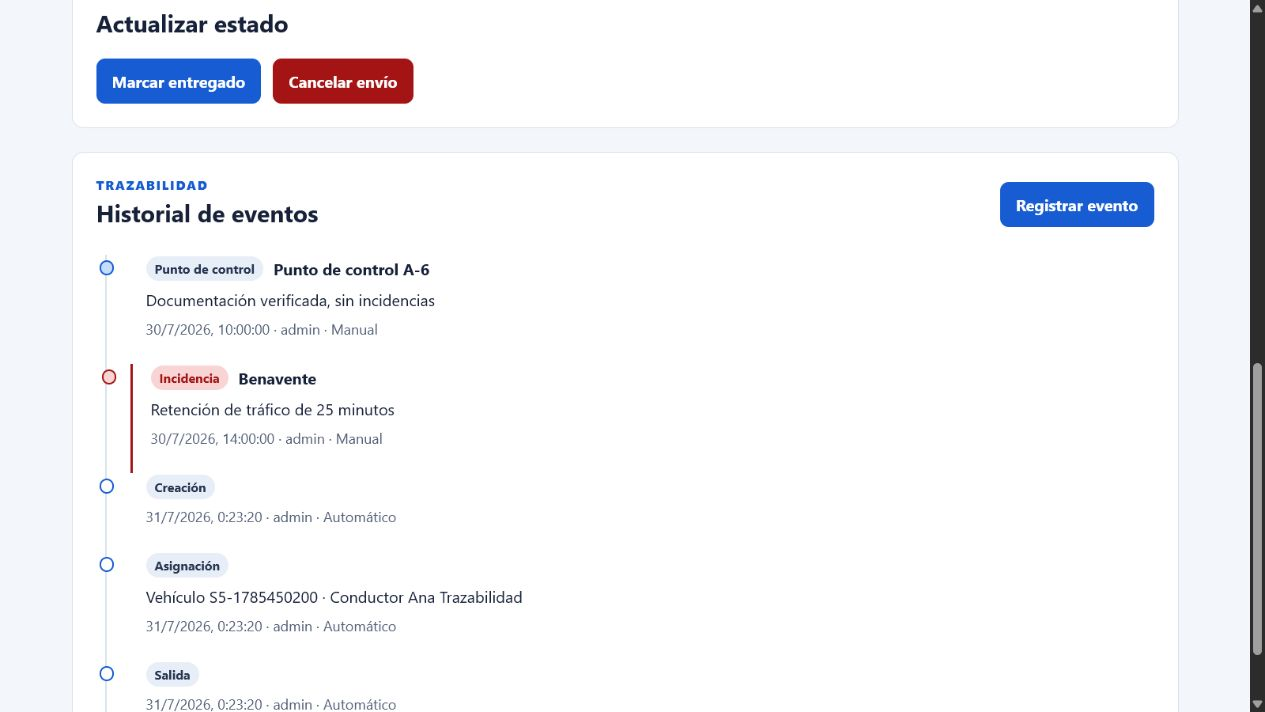
\includegraphics[width=\textwidth]{imaxes/historial-eventos-sprint5}
\caption{Línea de tiempo con eventos automáticos y manuales del Sprint 5}
\label{fig:historial-s5}
\end{figure}

\begin{figure}[htbp]
\centering
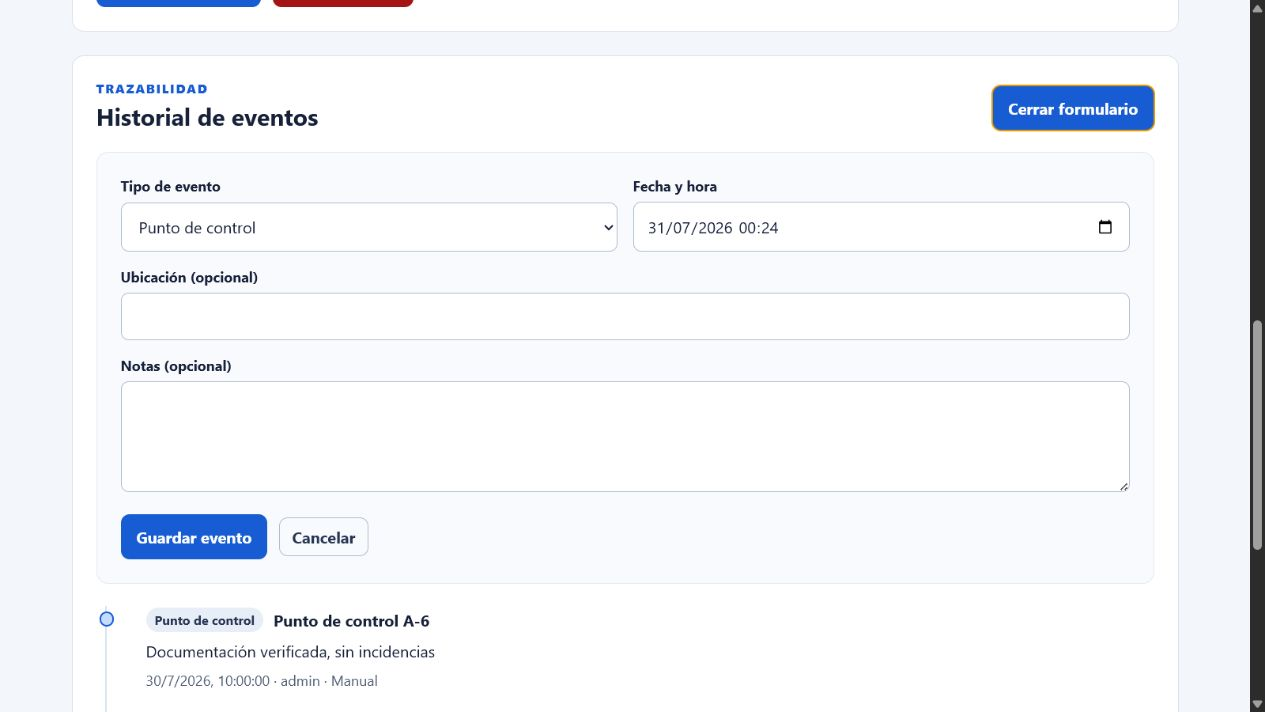
\includegraphics[width=0.78\textwidth]{imaxes/registro-evento-sprint5}
\caption{Formulario de registro de un evento manual}
\label{fig:registro-evento-s5}
\end{figure}

\clearpage
\section{Sprint 6: administración e indicadores}

El sexto incremento cerró los requisitos funcionales de prioridad media sin modificar el esquema. La entidad \texttt{AppUser}, diseñada y migrada en el Sprint 1, ya contenía rol, estado y marcas temporales; el resumen se obtiene mediante agregaciones sobre envíos y eventos. Esta ausencia de migración es un resultado del diseño anticipado del modelo, no una reducción de alcance.

La administración de usuarios se separó del servicio de autenticación y se situó tras la política \texttt{Admin}. Permite alta, cambio de rol, desactivación y reactivación, pero no borrado. Usuario y correo conservan unicidad global aunque la cuenta esté inactiva, porque identifican a la persona en el historial. RN-12 se aplica antes de cualquier mutación mediante una guarda común: desactivar al último administrador activo o degradarlo a operador devuelve un conflicto \texttt{last\_admin\_protected}. La SPA oculta el módulo a operadores y una ruta específica redirige también cualquier navegación directa; la API continúa siendo la autoridad y devuelve 403.

El cambio de contraseña propia reutiliza \texttt{ICurrentUser}: carga la cuenta activa, verifica el hash de la contraseña actual y rechaza tanto una credencial incorrecta como una nueva contraseña idéntica. El JWT no se sustituye ni se revocan sesiones previas. Del mismo modo, un token ya emitido sobrevive temporalmente a una desactivación o cambio de rol. Es una limitación consciente de la autenticación sin estado, acotada por la caducidad del token, que se revisará junto con el almacenamiento en \texttt{localStorage} durante el endurecimiento del Sprint 7.

El endpoint \texttt{/summary} combina tres consultas. Los contadores por estado son globales y representan la situación actual. La actividad de vehículo y conductor usa la fecha prevista de recogida dentro de un periodo configurable ---treinta días por defecto---, mientras que las incidencias se cuentan por \texttt{OccurredAt}. Las etiquetas se resuelven sin filtrar recursos inactivos, de modo que una baja no borra actividad histórica. En el Inicio de la SPA, cada contador enlaza al listado de envíos ya filtrado y la interfaz explica expresamente qué cifras dependen del periodo.

\begin{figure}[htbp]
\centering
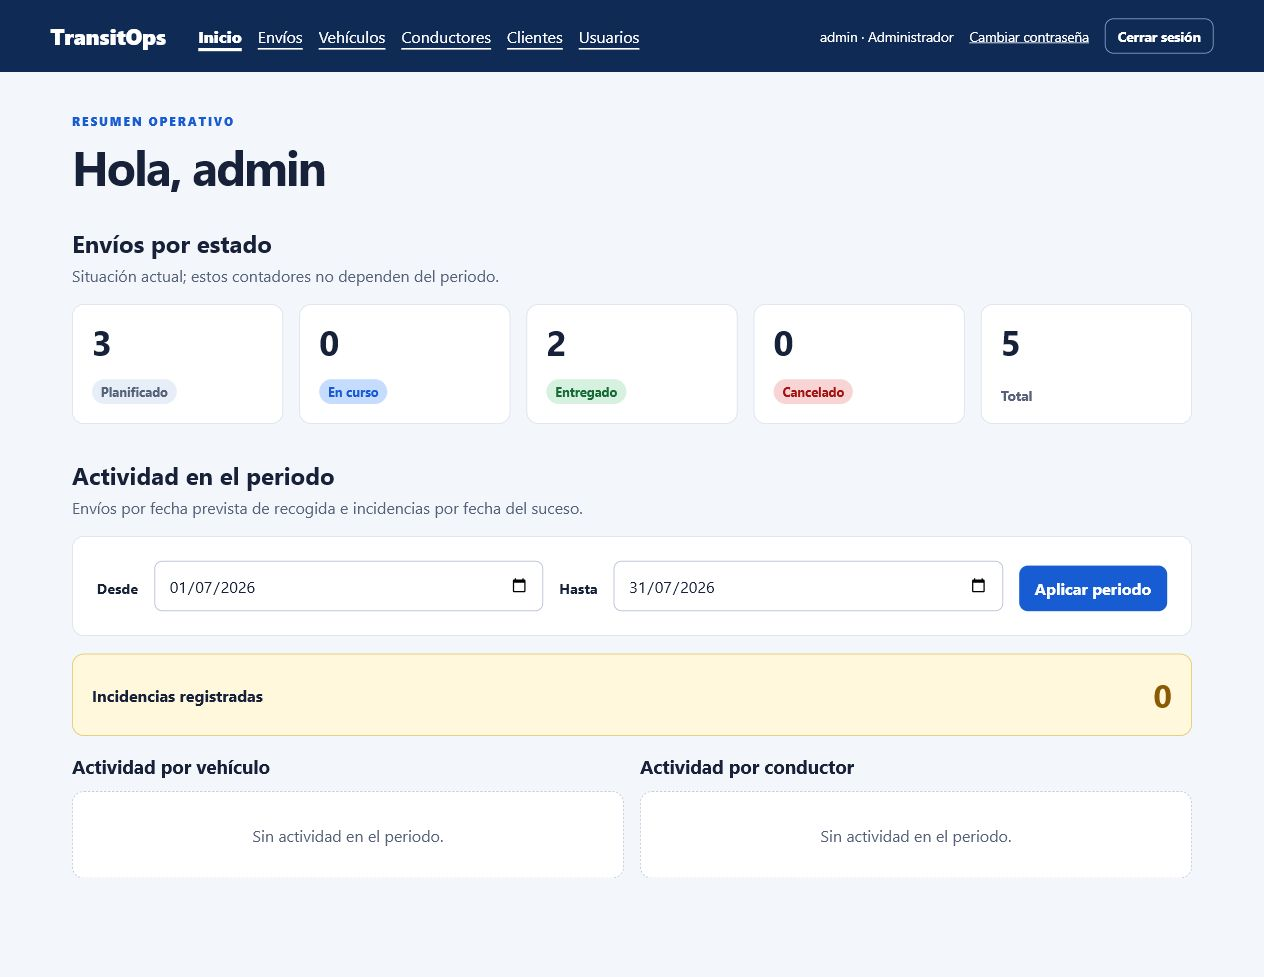
\includegraphics[width=\textwidth]{imaxes/resumen-sprint6}
\caption{Panel operativo con situación actual y actividad del periodo}
\label{fig:resumen-s6}
\end{figure}

\clearpage
\section{Sprint 7: endurecimiento, pruebas de sistema y despliegue}

Con RF-01--RF-14 implementados, el séptimo incremento no añadió funcionalidad sino que atacó lo que los seis anteriores habían dejado anotado como deuda. Por tamaño se dividió en cuatro tramos consecutivos, cada uno con su propio cierre, y el orden entre ellos respondió a una decisión concreta: las pruebas de sistema se escribieron \emph{antes} del cambio de sesión, para que actuasen como red de seguridad del refactor más invasivo. Al recorrer la interfaz, esas pruebas son indiferentes a si el token viaja en almacenamiento local o en una cookie; escritas después no habrían protegido nada.

\subsection*{Concurrencia sostenida por el motor}

El primer tramo cerró las dos carreras declaradas en los Sprints 4 y 6. La regla anti-doble-reserva pasó a estar garantizada por dos índices únicos parciales sobre los envíos, uno por vehículo y otro por conductor, limitados a los estados abiertos; la protección del último administrador se serializó con un cerrojo de aviso mantenido dentro de la transacción. La comprobación previa en el servicio se conservó en ambos casos, porque es la que produce un mensaje útil: el índice aporta corrección, el servicio aporta explicación.

Verificar esto obligó a ampliar la estrategia de pruebas. Ni un índice filtrado ni un cerrojo existen en el proveedor en memoria que usan las pruebas rápidas, así que se incorporó una clase que arranca PostgreSQL real en un contenedor efímero y lanza dos operaciones simultáneas. Es el primer punto del proyecto donde una regla no podía demostrarse sin pagar el coste de infraestructura de prueba.

\subsection*{Pruebas de sistema y dependencias}

El segundo tramo automatizó los cuatro flujos de negocio con Playwright sobre la composición de contenedores. Las pruebas son independientes entre sí y no reinician la base: generan datos únicos por ejecución, algo obligatorio y no cosmético, porque las credenciales de usuario y las referencias de envío son únicas de forma global e incluyen a los registros inactivos. El arranque del primer administrador, que solo puede tener éxito una vez por base de datos, se resolvió en la preparación global tolerando el conflicto.

La misma revisión abordó las dependencias del frontend. La auditoría encontró cinco avisos, uno de ellos en una dependencia de producción ---una vulnerabilidad de falsificación de petición en el enrutador--- y el resto en el árbol de desarrollo y pruebas. Se actualizaron por versiones compatibles en lugar de aplicar correcciones automáticas mayores, y se documentó el alcance de cada cadena para distinguir lo que llega a la imagen servida de lo que no.

\subsection*{Sesión endurecida}

El tercer tramo pagó la deuda más visible del Sprint 1. El token dejó de ser puramente autocontenido: incorpora una versión de sesión que se comprueba en cada petición protegida, de modo que cambiar la contraseña, desactivar la cuenta o modificar el rol invalidan de inmediato los tokens anteriores. Y el almacenamiento local dio paso a una cookie \texttt{HttpOnly} con \texttt{SameSite=Strict}, barata de adoptar porque la aplicación siempre ha operado en mismo origen.

El cambio tuvo dos consecuencias que no eran evidentes al planificarlo. La respuesta de acceso dejó de contener el token, lo que alteró el contrato y las pruebas que lo simulaban; y la interfaz perdió la capacidad de leer su propia sesión, de modo que necesitó un punto final nuevo para reconstruirla al recargar. Sin él, refrescar la página expulsaba al usuario. Ambas se descubrieron al implementar, no al diseñar, y quedan registradas porque ilustran el tipo de coste que un cambio de mecanismo arrastra más allá de su propia superficie.

\subsection*{Despliegue accesible}

El cuarto tramo llevó la aplicación a una máquina virtual Ubuntu con Docker Compose, accesible por una dirección HTTPS temporal mediante un túnel saliente, sin publicar ningún puerto ni abrir el router. La entrega quedó automatizada hasta el registro de contenedores y la máquina consume desde allí, con un temporizador que comprueba novedades cada cinco minutos. El Capítulo~\ref{chap:despliegue} detalla la topología y el procedimiento.

Cerrado ese tramo, una revisión completa del incremento localizó trece defectos de coherencia, ninguno funcional: en su mayoría código y configuración que el cambio de sesión había dejado sin uso pero aparentando seguir activos ---un punto final duplicado, una política de intercambio de recursos entre orígenes inservible, un ayudante de pruebas que leía un campo eliminado--- además de una vulnerabilidad de severidad alta que había entrado de forma transitiva con la infraestructura de pruebas del primer tramo. Doce se corrigieron; el restante, la no identidad entre las imágenes probadas y las publicadas, se documentó como limitación conocida. Que una revisión posterior encuentre este tipo de residuo es esperable cuando un sprint sustituye un mecanismo transversal, y registrarlo es más útil que presentar el incremento como limpio desde el principio.

\subsection*{Sprint 8 --- Cierre}

El último incremento consolida esta memoria, produce el material de defensa y revisa que la documentación del repositorio describa el sistema realmente entregado.
